\input{header.tex}

\begin{document}

\lecture{ 34 --- File Allocation Methods }{\term}{Jeff Zarnett}

\section*{File Allocation Methods}

Much like memory allocation, there is a need to choose a strategy for how to allocate disk space. There are three major ways that we could allocate the disk space to files: contiguous, linked, and indexed; each has its advantages and disadvantages.

\subsection*{Contiguous Allocation}
The contiguous allocation strategy means that a file occupies a set of contiguous blocks on disk. So a file is allocated, starting at block $b$ and is $n$ blocks in size, the file takes up blocks $b, b+1, b+2, ..., b+(n-1)$. This is advantageous, because if we want to access block $b$ on disk, accessing $b+1$ requires no head movement, so seek time is nonexistent to minimal (if we need to move to another cylinder). 

All that we need to maintain are the values of $b$ and $n$: the start location and length of the file. Both sequential and direct access are very easy: the first block of a file is at $b$. To access a block $i$ at some offset into the file, it is simply at the base address $b$ plus $i$. Checking if the access is valid is also an easy operation: if $i < n$ then it is valid.

See the diagram below to get an example of contiguous allocation:
\begin{center}
	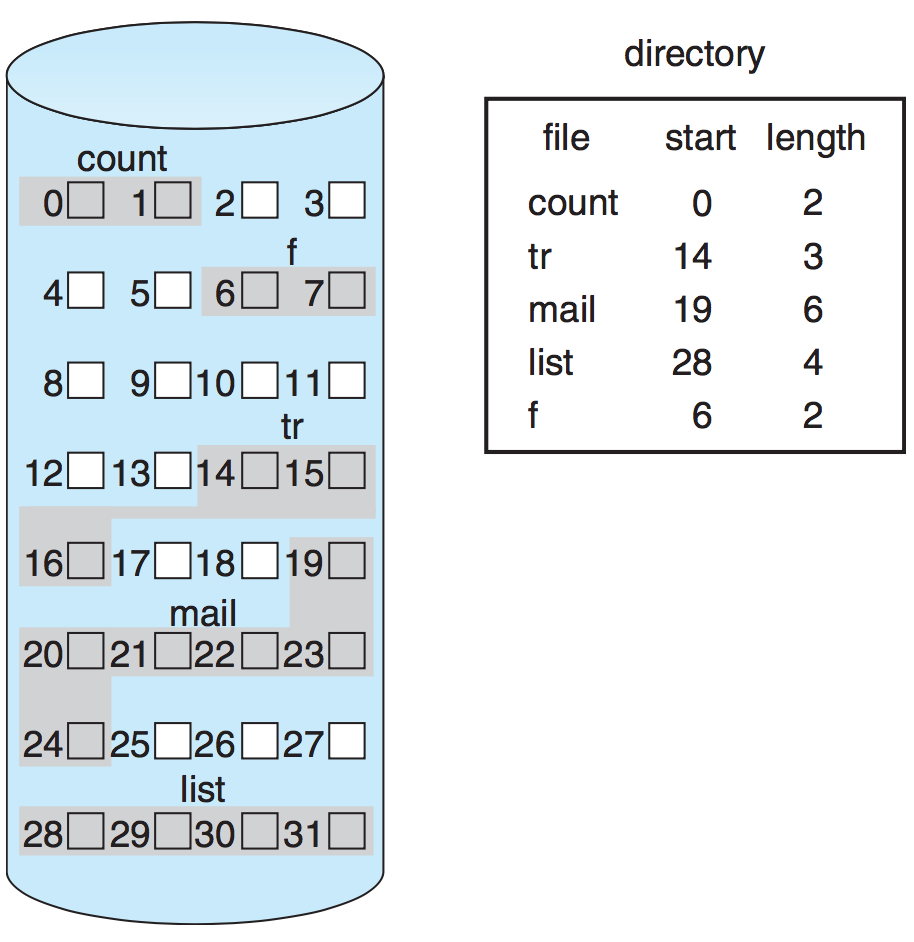
\includegraphics[width=0.4\textwidth]{images/disk-contiguous.png}\\
	Contiguous allocation of disk space~\cite{osc}.
\end{center}

This takes us back to a problem we have seen once before: the memory allocation problem. If we need a memory block of size $N$: (1) can we find a contiguous block of $N$ or greater to meet that allocation? and (2) if there is more than one block, which one do we choose? As before, we suffer the problem of external fragmentation, plus a bit of internal fragmentation in the last block of the file. 

There was also talk on the subject of memory allocation of compaction. This was moving memory allocations around in memory to create some larger free spaces that can be allocated. But for languages like C, it was not realistic, because of the impossibility of updating all pointers (unlike Java where we can update all references). We can do compaction on disk, but it takes a very, very long time and is computationally expensive. Doing compaction can be done when the system has nothing else to do (idle priority operation) or on some schedule when it would be minimally disruptive (e.g., middle of the night... mind you... a lot of programmers do most of their work in the middle of the night...).

Another problem, of course, with contiguous allocation is that old clairvoyance issue: how much space is a file going to take? If it is just a copy-paste operation, the copy is the same size as the original, so there is no problem. When a user opens a new document, how does the OS know how big the file is going to be? Is this a 3 page essay or a 300 page thesis? If we allocate too little space, we may be able to tack on space at the end, or that block may be allocated, forcing us to move the file and reallocate it. If the value we choose is too large, then ~\cite{osc}.

\subsection*{Linked Allocation}
Linked allocation is a solution to the problems of contiguous allocation: instead of a file being all in consecutive blocks, the we maintain a linked list of the blocks, and the blocks themselves may be located anywhere on the disk. The directory listing just has a pointer to the first and lack blocks (head and tail of the linked list).

If a new file is created, it will be created with size zero and the head and tail pointers are null. When a new block is needed, it can come from anywhere and will just be added to the linked list. Thus, compaction and relocation are not really an issue. Unfortunately, however, accessing block $i$ of a file is no longer as simple as computing an offset from the first block; it requires following $i$ pointers (a pain).

\begin{center}
	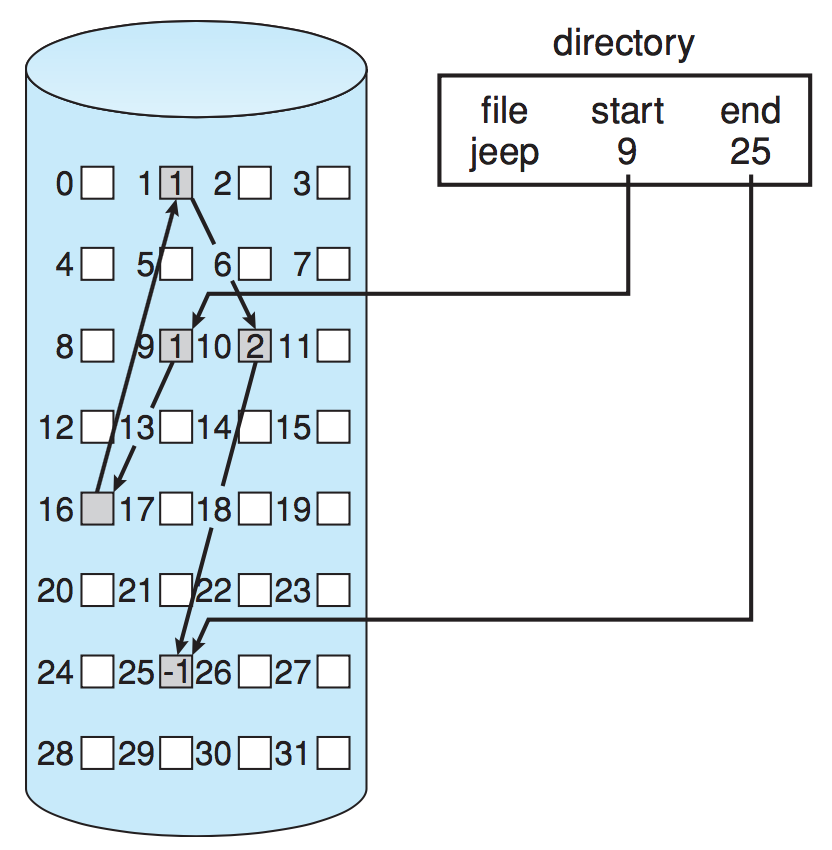
\includegraphics[width=0.4\textwidth]{images/disk-linked.png}\\
	Linked allocation of disk space~\cite{osc}.
\end{center}

A possible solution to the problem of following so many pointers (and the overhead of maintaining so many) is to group up the blocks into \textit{clusters}, where a cluster is comprised of, say, four blocks. Then we waste less memory maintaining pointers and it improves disk accesses because there is less seeking back and forth to various disk locations~\cite{osc}. 

One variation of linked allocation is the File Allocation Table (FAT), which was used by the MS-DOS operating system (FAT16 and FAT32 were used in Windows before NTFS came in with NT/2000/XP and their descendants). The FAT32 file system hangs on these days as the file system of choice for formatting USB flash drives because it means the data will be readable in Windows, Mac OS X, and Linux. This is primarily because Microsoft has not made the NTFS file system standard public and Windows systems do not support too many other file systems, and Windows has such a big marketshare. So the FAT32 option is used, despite its known problems (and limitations, like 4~GB max file size), because it's the one system everyone can understand. Isn't the state of personal computing so... uplifting?

The FAT allocation scheme works like this: at the beginning of the disk, there is a table to maintain file allocation data (hence the name). The table has one entry for each block and is indexed by block number. It works like a linked list; the directory entry has the first block of the file and the table entry under that block number has the index of the next block. The chain continues until the last block where there is a special end-of-file value. An unused block has a table value of 0. Thus, to allocate a new block, find the first 0-valued entry, and replace the previous end-of-file value with the address of the new block~\cite{osc}. See the example below:


\begin{center}
	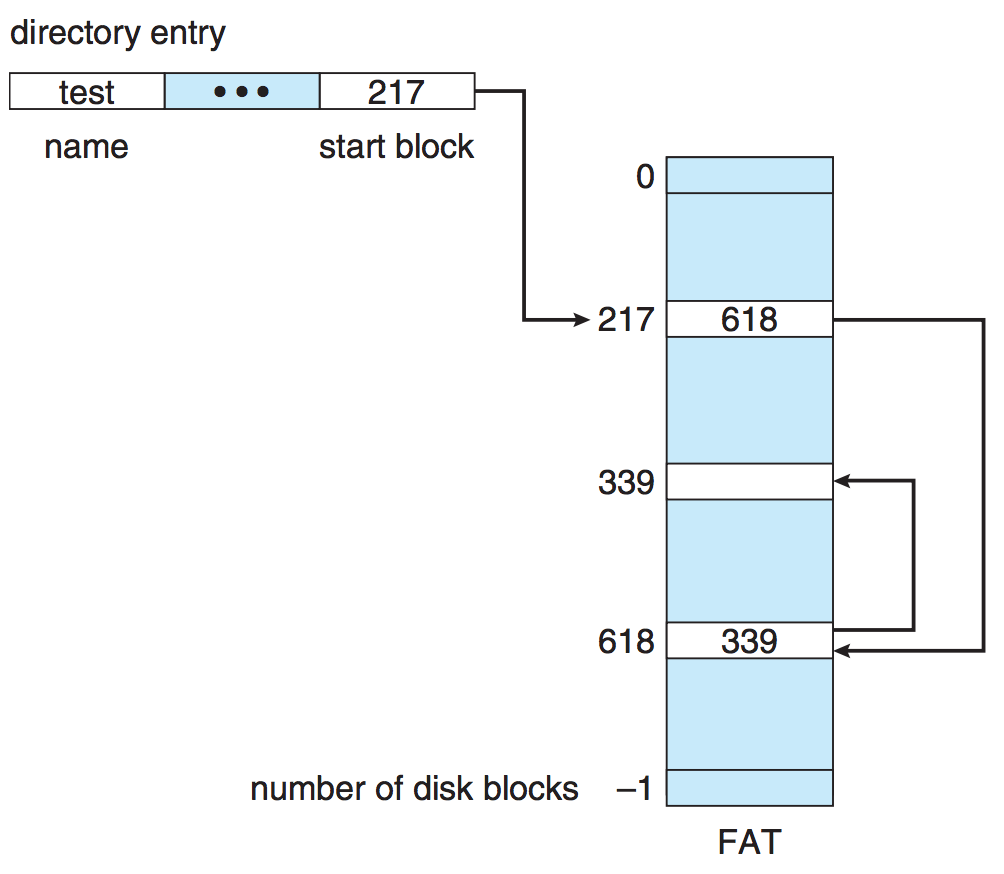
\includegraphics[width=0.5\textwidth]{images/file-allocation-table.png}\\
	File Allocation Table (FAT)~\cite{osc}.
\end{center}

The FAT itself should be cached in memory, otherwise the disk is going to have to seek back to it unbearably often.

\subsection*{Indexed Allocation}
If we stuck to pure linked allocation, we still have the problem that accessing some part in the middle of the file is a pain because we have to follow and retrieve a lot of pointers to the different blocks. The idea of indexed allocation is to take all the pointers and put them into one location: an index block. So, the first block of the file contains a whole bunch of pointers. To get to block $i$, just go to index $i$ of the index block and we can get the location of block $i$ much more efficiently than we could in linked allocation. All pointers to blocks start as null, and when we add a new block, add its corresponding entry into the index block~\cite{osc}. See the diagram below:

\begin{center}
	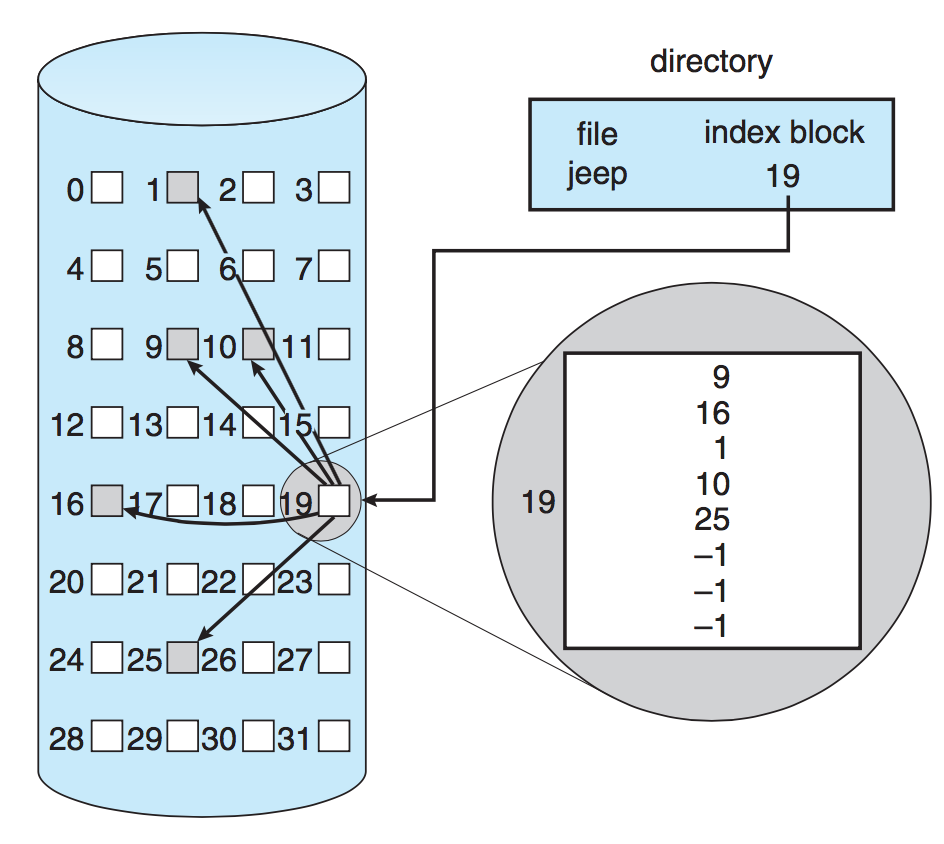
\includegraphics[width=0.4\textwidth]{images/disk-indexed.png}\\
	Indexed allocation of disk space~\cite{osc}.
\end{center}

Like many of the other systems we have examined, there is a need to make a decision about the size of a block. If a file needs only 1-2 blocks, one whole block is allocated for the pointers which contains only 1-2 entries. That suggests we want the index to be small, but what if we need more pointers than fit into one block? There are a few mechanisms for this~\cite{osc}:

\begin{enumerate}
	\item \textbf{Linked Scheme}: An index block is a disk block, and we can link together several index blocks. The last entry in the index block is either null or a pointer to the next index block.
	\item \textbf{Multilevel Index}: A variant of the linked scheme that has multiple levels. The first level block points to the second level block; the second level block points to the actual file data. This can go to as many levels are necessary based on the maximum file size. If a block is 4~KB, we can have 1024 4-byte pointers, so two levels would allow a maximum file size of up to 4~GB.
	\item \textbf{Combined Scheme}: The all-of-the-above option. This is used in UNIX. Keep the first 15 pointers of the index block in the inode structure; 12 of them point directly to file data. The next three pointers refer to indirect blocks. The 13th is an index block containing the addresses of blocks with data. The 14th points to a double indirect block (addresses of blocks containing addresses of blocks). The 15th points to a triple indirect block\footnote{Yo dawg, we heard you like index blocks...}.
\end{enumerate}

With that out of the way, we can finally show a visual representation of an inode.

\begin{center}
	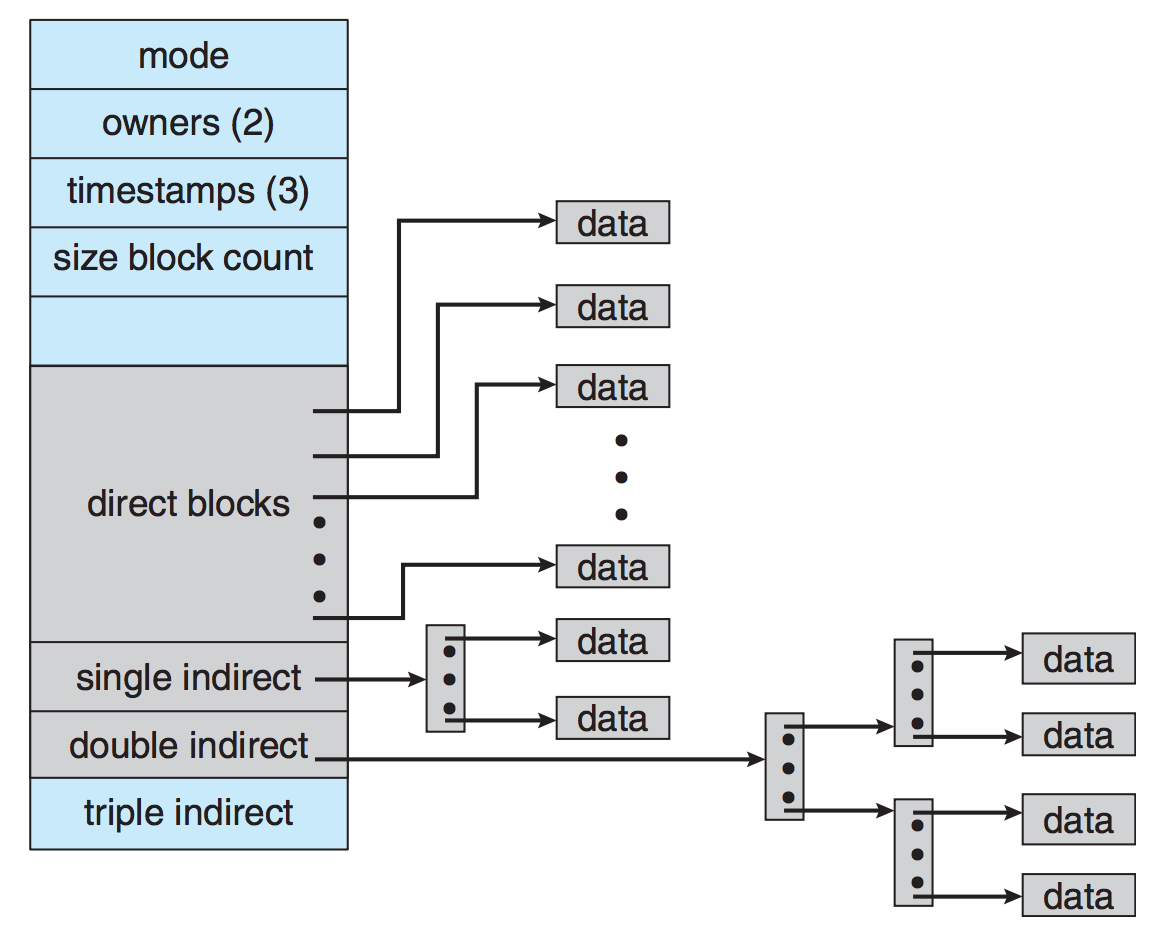
\includegraphics[width=0.6\textwidth]{images/unix-inode.png}\\
	The UNIX inode. Triple indirection is left to the reader's imagination~\cite{osc}.
\end{center}

\subsection*{Other Disk Issues}
As with memory, the system will keep track of the free space available.

Bit vectors work just the way we would expect: create a structure in memory where a bit represents a block. If it is free, the bit is 1; allocated is 0. So a bit vector looks like \texttt{0100110111011111000000...}. The problem with this strategy is, of course, that the bigger the disk, the more overhead is needed to store this bit vector.

The next rather obvious approach is a linked list: the head points to the first free space block, and we can traverse the list to get to the next free block. See the diagram below:

\begin{center}
	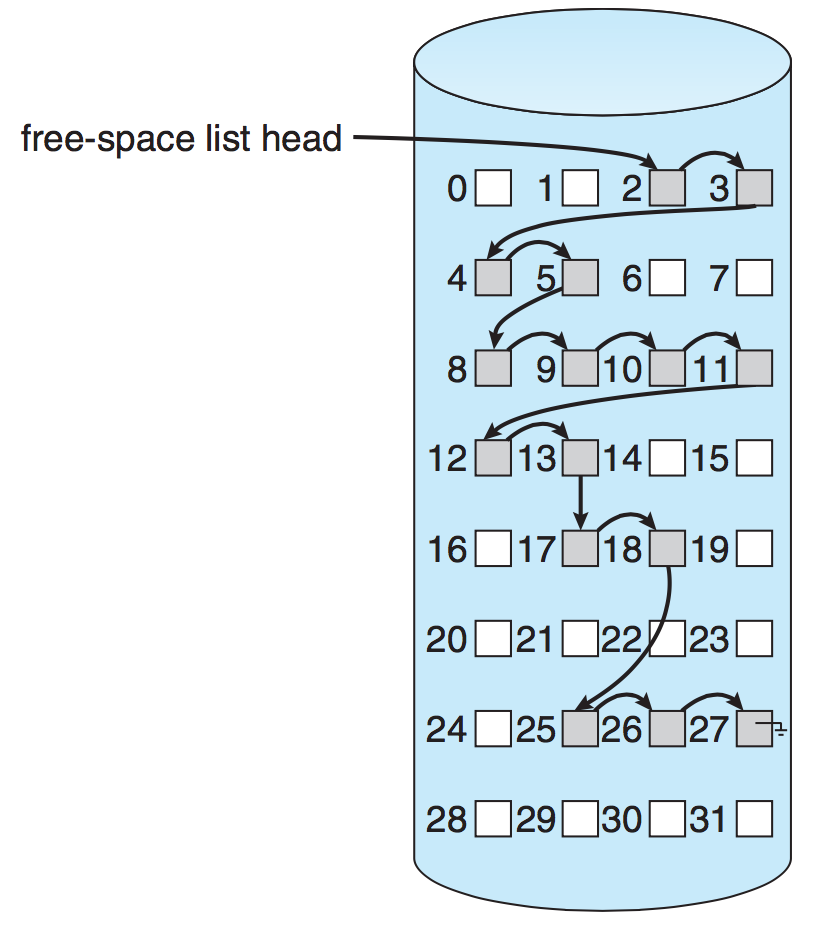
\includegraphics[width=0.4\textwidth]{images/disk-linked-list.png}\\
	Linked free-space list on disk~\cite{osc}.
\end{center}

Grouping makes this slightly more interesting: the first free block will be used to store the addresses of $n$ free blocks, the first $n-1$ of which are actually free. The last block contains a block with another set of $n$ free blocks. So if we need a large number of free blocks, we can find them quickly, instead of walking through the list one block at a time, which takes a lot of disk accesses. Counting is a slight improvement on this where we also store a number $k$ of free contiguous blocks after each address. So, if block 27 is followed by three consecutive free blocks, instead of having 27, 28, 29, 30 as entries, it will show (27, 4). The entries may be stores in a balanced tree for efficient operations~\cite{osc}.


The efficient use of a disk depends on the disk-allocation and directory algorithms. UNIX inodes, for example, are preallocated, so even a disk containing no files has some of its space taken up by the inodes. Preallocation of inodes and distribution of them improves the file system performance, because the UNIX allocation and free-space algorithms keep the file data near the inode, where possible, to reduce seek time~\cite{osc}.

\subsection*{Consistency Checking and Journalling}

Unfortunately, an error, crash, or power failure or something similar may result in a loss of data or inconsistent data in the file system. The directory structures, pointers, inodes, FCBs, et cetera are all data structures and if they become corrupted it may lead to serious problems.

We could check for inconsistent data periodically (e.g., on system boot up) and many operating systems do so. This is, of course, an operation that will consume a very large amount of time while the whole disk is scanned. The UNIX tool for this is \texttt{fsck} (... not exactly something you want to say out loud) and the Windows tool is \texttt{chkdsk} (check disk). These tools will look for inconsistent states (e.g., a file that claims to be 12 blocks but the linked list contains only 5) and will attempt to repair the data structures. Its level of success depends on the nature of the problem and the implementation of the file system.

Obviously we would like to prevent the problem, if we can. Recall from much earlier the concept of atomic operations: an operation should either succeed completely, or not take place at all. Your first experience with such a structure may have been in version control, when using subversion: either a commit takes place in its entirety or it is as if it never happened. This approach is used in the Windows NTFS system as well as Mac OS HFS+ (if journalling is enabled). 

Though we might be familiar, at this point, with the concept of the \textit{transaction}, now let us take a moment to see how it actually works. The simple explanation is: before making any changes, make a list of all the things we plan to do. Then do the things written down. Then we consider the transaction complete.

All metadata changes are written sequentially to a log file; once the changes are written to the log, control may return to the program that requested the operation. Meanwhile, the log entries are actually carried out. As changes are made, a pointer is updated to indicate which of the log entries have really happened and which have not. When an entire transaction is completed, it is removed from the log file. If the system crashes, the log file will contain zero or more transactions. If there are zero there is no problem: nothing was in progress at the time of the crash. If there are some, then the transactions were not completed and the operations should still be carried out. If a transaction was aborted (not committed), we walk backwards through the log entries to undo any completed operations and go back to the state before the start of the transaction~\cite{osc}.

Even though a particular write may not have taken place because of a crash, resulting in some data loss, at least the system will always remain in a consistent state. As a side benefit, we can sometimes re-order the writes to get better performance (e.g., schedule them in such a way that we get better disk utilization). 

The approach in the Solaris ZFS approach is similar, but not identical. Blocks are never overwritten with new data. Instead, a transaction writes all data and metadata to new blocks. Only when the transaction is complete, any references to the old blocks are replaced with the location of the new blocks. Then the old pointers and blocks can be cleaned up (reused or disposed of). 

\subsection*{Backups}

One final note about hard disk drives. We often think of them as places for permanent storage of data, but hard drives can and do fail. So please, take backups of important data.

\input{bibliography.tex}

\end{document}